\documentclass[12pt,a4paper]{article}
\usepackage[utf8]{inputenc}
\usepackage[spanish,es-tabla]{babel}
\usepackage{geometry}
\usepackage{graphicx}
\usepackage{multirow}
\usepackage{tabularx}
\usepackage{mathptmx}
\usepackage{fancyhdr}
\usepackage{array}
\usepackage[table]{xcolor}
\usepackage{titlesec}
\usepackage{setspace}
\usepackage{microtype}
\usepackage{lastpage}
\usepackage{booktabs}
\usepackage{enumitem}
\usepackage{amsmath}
\usepackage{amsfonts}
\usepackage{amssymb}

\usepackage{float}
\usepackage{placeins}
\usepackage{tikz}
\usepackage{pgfplots}
\pgfplotsset{compat=1.17}
\usetikzlibrary{arrows.meta,positioning,shapes.geometric,calc}

\graphicspath{{images/}{../images/}{./}}

\geometry{
    top=4.7cm,
    bottom=2.5cm,
    left=2.5cm,
    right=2.5cm,
    headheight=3.9cm,
    headsep=0.4cm
}

\setstretch{1.15}
\setlength{\parindent}{0pt}
\setlength{\parskip}{0.45em}
\setlength{\tabcolsep}{4pt}

\titleformat{\section}
  {\normalfont\fontsize{12}{14.5}\bfseries}{\thesection.}{0.6em}{\uppercase}
\titlespacing*{\section}
  {0pt}{1.8ex plus 0.4ex minus 0.2ex}{0.6ex plus 0.2ex}

\titleformat{\subsection}
  {\normalfont\fontsize{11.5}{13.5}\bfseries}{\thesubsection.}{0.5em}{}
\titlespacing*{\subsection}
  {0pt}{1.4ex plus 0.3ex minus 0.1ex}{0.4ex plus 0.1ex}

\titleformat{\subsubsection}
  {\normalfont\fontsize{10.5}{12.5}\bfseries\itshape}{\thesubsubsection.}{0.4em}{}
\titlespacing*{\subsubsection}
  {0pt}{1.1ex plus 0.2ex minus 0.1ex}{0.3ex plus 0.1ex}

\newcolumntype{Y}{>{\centering\arraybackslash}X}
\newcolumntype{L}{>{\raggedright\arraybackslash}X}
\newcolumntype{C}{>{\centering\arraybackslash}X}

\definecolor{headerblue}{RGB}{26, 54, 93}
\definecolor{darkblue}{RGB}{43, 108, 176}
\definecolor{lightgraybg}{RGB}{248, 248, 248}
\definecolor{tableheader}{RGB}{232, 238, 246}
\definecolor{navyheader}{RGB}{0, 32, 96}
\definecolor{lineblue}{RGB}{0, 102, 204}
\definecolor{areablue}{RGB}{220, 236, 252}
\definecolor{lcsred}{RGB}{217, 56, 41}
\definecolor{lcigreen}{RGB}{46, 125, 50}
\definecolor{lciorange}{RGB}{230, 81, 0}
\definecolor{ishikawared}{RGB}{160, 0, 0}

\tikzset{
    catbox/.style={draw, fill=tableheader, font=\footnotesize\bfseries, minimum width=2.8cm, minimum height=0.65cm, align=center},
    efectobox/.style={draw=ishikawared!90!black, line width=1.2pt, fill=ishikawared, text=white, font=\small\bfseries, align=center, inner sep=6pt, text width=3.8cm},
    causetext/.style={font=\scriptsize, align=right, text=black!90}
}

\newcommand{\docCodigo}{TI-SIGE-ENT-F2-003}
\newcommand{\docVersion}{1.0}
\newcommand{\docProceso}{DISEÑO DETALLADO DE SOFTWARE / UML DINÁMICO Y ESTÁTICO}
\newcommand{\docElaboracion}{26/08/2026}
\newcommand{\docRevision}{26/08/2026}
\newcommand{\docTitulo}{DIAGRAMAS DE SECUENCIA, ACTIVIDADES Y CLASES}
\newcommand{\docOrganizacion}{FACULTAD DE INGENIERÍA EN SISTEMAS, ELECTRÓNICA E INDUSTRIAL}
\newcommand{\docSubOrganizacion}{CARRERA DE INGENIERÍA DE SOFTWARE}

\newcommand{\encabezadofrecuente}{%
    \renewcommand{\arraystretch}{1.15}%
    \noindent\makebox[\textwidth][c]{%
    \begin{tabularx}{\textwidth}{|>{\centering\arraybackslash}m{2.8cm}|Y|>{\centering\arraybackslash}m{4.8cm}|}
        \hline
        \multirow{4}{2.8cm}{\centering\raisebox{-1.15cm}{
\includegraphics[width=2.5cm,height=2.0cm,keepaspectratio]{images/logo.png}}}
        & \textbf{\fontsize{9}{11}\selectfont \docOrganizacion} 
        & \textbf{\fontsize{8}{10}\selectfont CÓDIGO:} \fontsize{8}{10}\selectfont \docCodigo \\
        \cline{3-3}
        & \textbf{\fontsize{8.5}{10.5}\selectfont \docSubOrganizacion} 
        & \textbf{\fontsize{8}{10}\selectfont VERSIÓN:} \fontsize{8}{10}\selectfont \docVersion \\
        \cline{2-3}
        & \textbf{\fontsize{8}{10}\selectfont PROCESO:} \fontsize{8}{10}\selectfont \docProceso 
        & \textbf{\fontsize{8}{10}\selectfont ELABORACIÓN:} \fontsize{8}{10}\selectfont \docElaboracion \\
        \cline{2-3}
        & \textbf{\fontsize{8.5}{10.5}\selectfont \docTitulo} 
        & \textbf{\fontsize{8}{10}\selectfont ÚLTIMA REVISIÓN:} \fontsize{8}{10}\selectfont \docRevision \\
        \hline
    \end{tabularx}%
    }%
}

\pagestyle{fancy}
\fancyhf{}
\fancyhead[C]{\encabezadofrecuente}
\fancyfoot[C]{\fontsize{10}{12}\selectfont Página \thepage\ de \pageref{LastPage}}
\renewcommand{\headrulewidth}{0pt}

\begin{document}

\noindent{\fontsize{10.5}{12.5}\selectfont \textbf{Integrantes:} Heidi Villavicencio \quad$\vert$\quad Steeven Toala \quad$\vert$\quad Nixon Hurtado \quad$\vert$\quad Andrea Vásquez}

\vspace{0.25cm}

\section{Título}
\textbf{Denominación Oficial del Entregable:} Diagramas de Secuencia, Actividades y Clases de Dominio -- Código EDT: 2.3

\section{Introducción}
El comportamiento dinámico y estructural de los componentes del sistema SIGE debe ser modelado de manera unívoca para guiar la etapa de desarrollo sin ambigüedades. Mientras que el diseño arquitectónico define las capas de alto nivel, los diagramas de secuencia, actividades y clases de dominio modelan el flujo de datos temporal, los caminos de decisión lógica y la estructura orientada a objetos de las entidades del Sistema de Gestión de Calidad (SGC). El presente documento captura las especificaciones detalladas para los flujos críticos de validación transaccional, ciclo de revisión en comités y modelo estático de clases bajo estándar OMG UML 2.5.1.

\section{Objetivo}
\subsection{Objetivo General}
Modelar detalladamente los flujos dinámicos de ejecución, las secuencias de interacción temporal y la estructura de clases de dominio del sistema SIGE mediante diagramas formales UML.
\subsection{Objetivos Específicos}
\begin{itemize}[leftmargin=1.5em, itemsep=2pt]
    \item Elaborar el Diagrama de Secuencia para el guardado y ejecución de Validation Gates.
    \item Modelar el Diagrama de Actividades para el ciclo completo de aprobación y revisión por comités.
    \item Estructurar el Diagrama de Clases de Dominio que mapea entidades, agregados y value objects institucionales.
\end{itemize}

\section{Alcance}
\subsection{Límites del Entregable (In-Scope)}
\begin{itemize}[leftmargin=1.5em, itemsep=2pt]
    \item Modelado de transacciones entre capas de Controlador, Servicio, Validación Gate y Repositorio.
    \item Mapeo exhaustivo del ciclo de vida de los estados del documento institucional.
    \item Definición de operaciones de negocio, visibilidad y multiplicidad de clases.
\end{itemize}
\subsection{Exclusiones (Out-of-Scope)}
\begin{itemize}[leftmargin=1.5em, itemsep=2pt]
    \item Clases auxiliares o utilitarias de rendering visual en React.
    \item Consultas SQL físicas (delimitadas en EDT 2.4).
\end{itemize}

\section{Definiciones}
\begin{itemize}[leftmargin=1.5em, itemsep=2pt]
    \item \textbf{Diagrama de Secuencia UML:} Diagrama de interacción que enfatiza el ordenamiento temporal de los mensajes enviados entre líneas de vida de objetos.
    \item \textbf{Diagrama de Actividades UML:} Representación gráfica del flujo de control o flujo de datos paso a paso entre actividades operacionales.
    \item \textbf{Diagrama de Clases de Dominio:} Modelo estructural que describe los tipos de objetos del sistema y las relaciones estáticas entre ellos.
    \item \textbf{Agregado (DDD):} Agrupación de objetos de dominio vinculados que se tratan como una unidad indivisible para el control de cambios de datos.
\end{itemize}

\section{Responsabilidades}
\begin{itemize}[leftmargin=1.5em, itemsep=2pt]
    \item \textbf{Steeven Toala (Responsable EDT 2.3):} Modelado de diagramas de secuencia e interacciones dinámicas.
    \item \textbf{Andrea Vásquez (Diseñadora de Procesos):} Modelado del diagrama de actividades y flujos de revisión.
    \item \textbf{Nixon Hurtado (Analista de Dominio):} Definición de clases de dominio, invariantes y métodos.
    \item \textbf{Ing. Paulo Torres (Docente Evaluador):} Verificación y aprobación técnica de los diagramas UML.
\end{itemize}

\section{Normativa Legal y Técnica}
\subsection{Marco Legal Ecuatoriano}
\begin{itemize}[leftmargin=1.5em, itemsep=2pt]
    \item \textbf{Ley Orgánica de Educación Superior (LOES), Art. 122:} Transparencia procedimental en la aprobación colegiada de planes académicos.
    \item \textbf{Reglamento de Régimen Académico (RRA - CES), Art. 45:} Fases secuenciales de planificación semestral y presentación de evidencias.
\end{itemize}
\subsection{Normas Técnicas Internacionales}
\begin{itemize}[leftmargin=1.5em, itemsep=2pt]
    \item \textbf{OMG UML 2.5.1 Specification:} Estándares para diagramas de secuencia, actividades y clases.
    \item \textbf{Domain-Driven Design (DDD) Reference (Eric Evans):} Patrones para el modelado de entidades y agregados ricos.
    \item \textbf{ISO/IEC 19505-1:2012:} Información y modelos conceptuales para arquitecturas de software.
\end{itemize}

\section{Método, Políticas y Contenidos}
\subsection{Enfoque Metodológico}
Se estructuraron los modelos dinámicos aplicando el principio de diseño por contratos. El Diagrama de Secuencia captura el flujo síncrono desde el envío HTTP del cliente React hasta la confirmación de la transacción en PostgreSQL, pasando obligatoriamente por la capa de validación de reglas de negocio (\textit{Validation Gate Pipeline}). El Diagrama de Actividades modela los caminos paralelos y bifurcaciones condicionales que determinan el avance hacia el Consejo Directivo o el retorno al docente elaborador por observaciones. El Diagrama de Clases formaliza el núcleo de entidades del dominio SGC.

\subsection{Políticas de Calidad del Modelado Dinámico}
\begin{enumerate}[leftmargin=1.5em, itemsep=2pt]
    \item \textbf{Política de Consistencia de Estados:} El estado de un documento solo puede transicionar mediante eventos explícitos y autorizados, impidiendo saltos directos no homologados.
    \item \textbf{Política de Transaccionalidad ACID:} Las operaciones que involucren el documento y su matriz de actividades deben ejecutarse bajo un único bloque transaccional atómico.
    \item \textbf{Política de Tipado Fuerte de Dominio:} Las clases de dominio deben encapsular sus atributos mediante métodos de negocio evitando modelos anémicos.
    \item \textbf{Política de Inmutabilidad de Firmas:} Una vez que un registro de firma es emitido, la clase \texttt{FirmaDocumento} pasa a ser inmutable en el dominio.
\end{enumerate}

\begin{figure}[H]
    \centering
    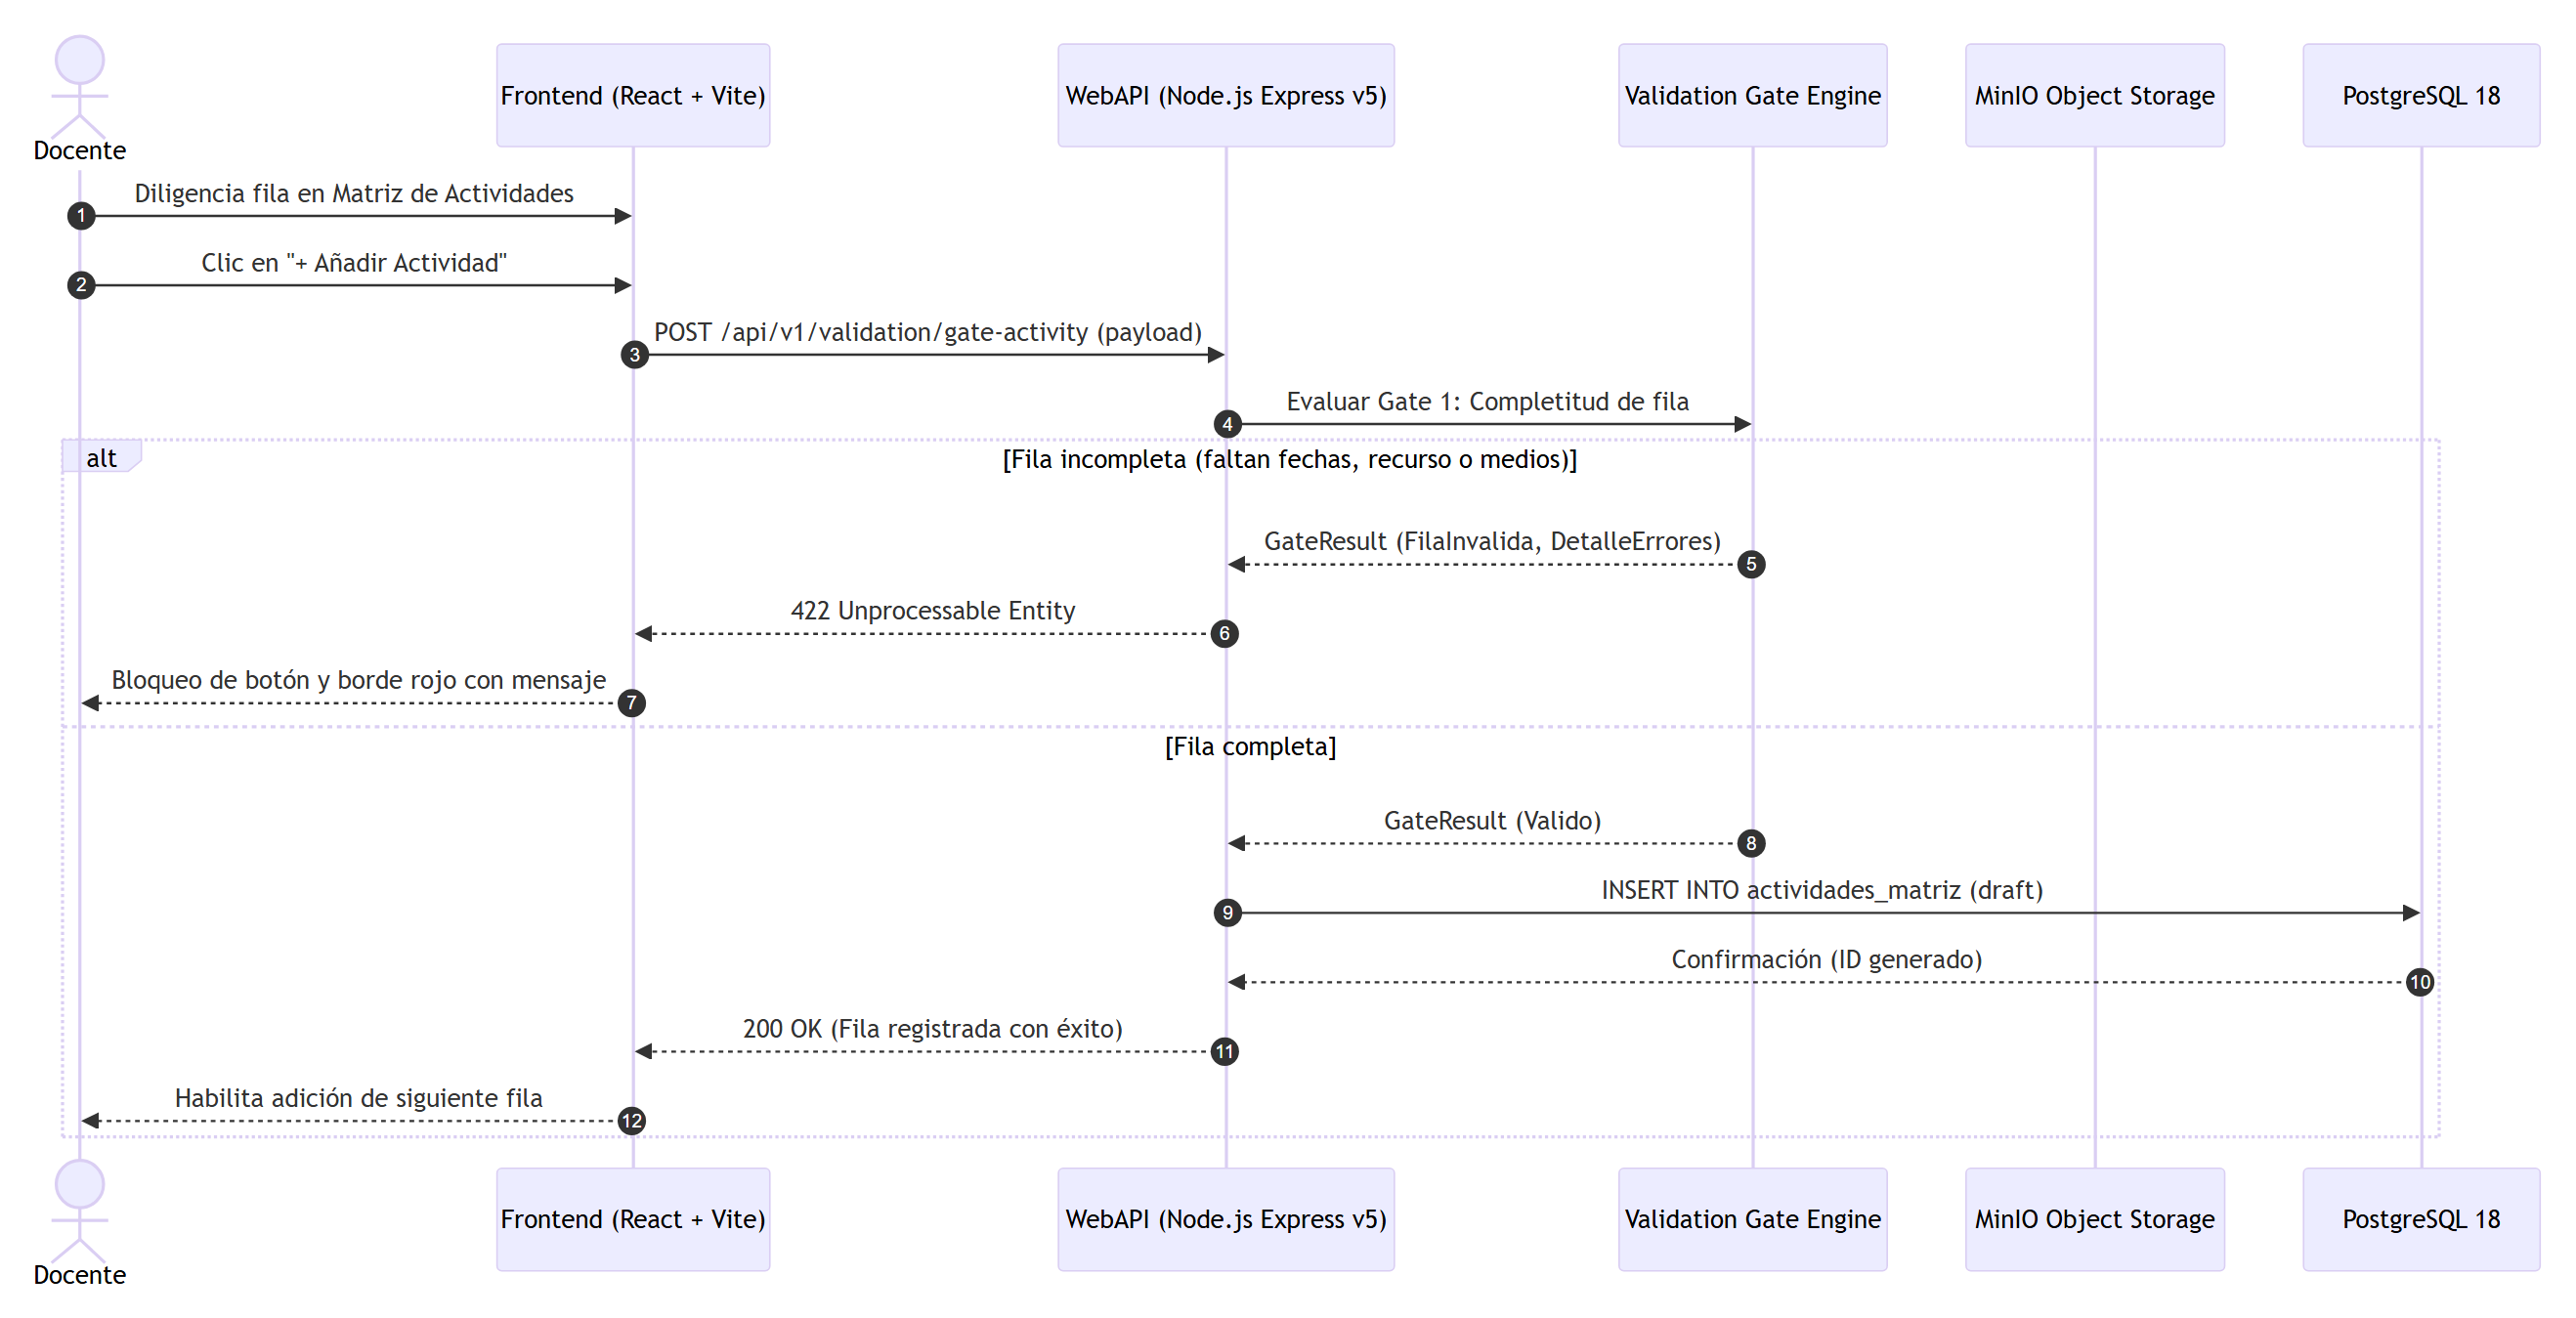
\includegraphics[width=0.88\textwidth,height=5.8cm,keepaspectratio]{images/s2_03_secuencia_validation.png}
    \caption{Diagrama de Secuencia UML: Guardado de Secciones y Evaluación de Validation Gates.}
    \label{fig:secuencia_gates}
\end{figure}
\FloatBarrier

\begin{figure}[H]
    \centering
    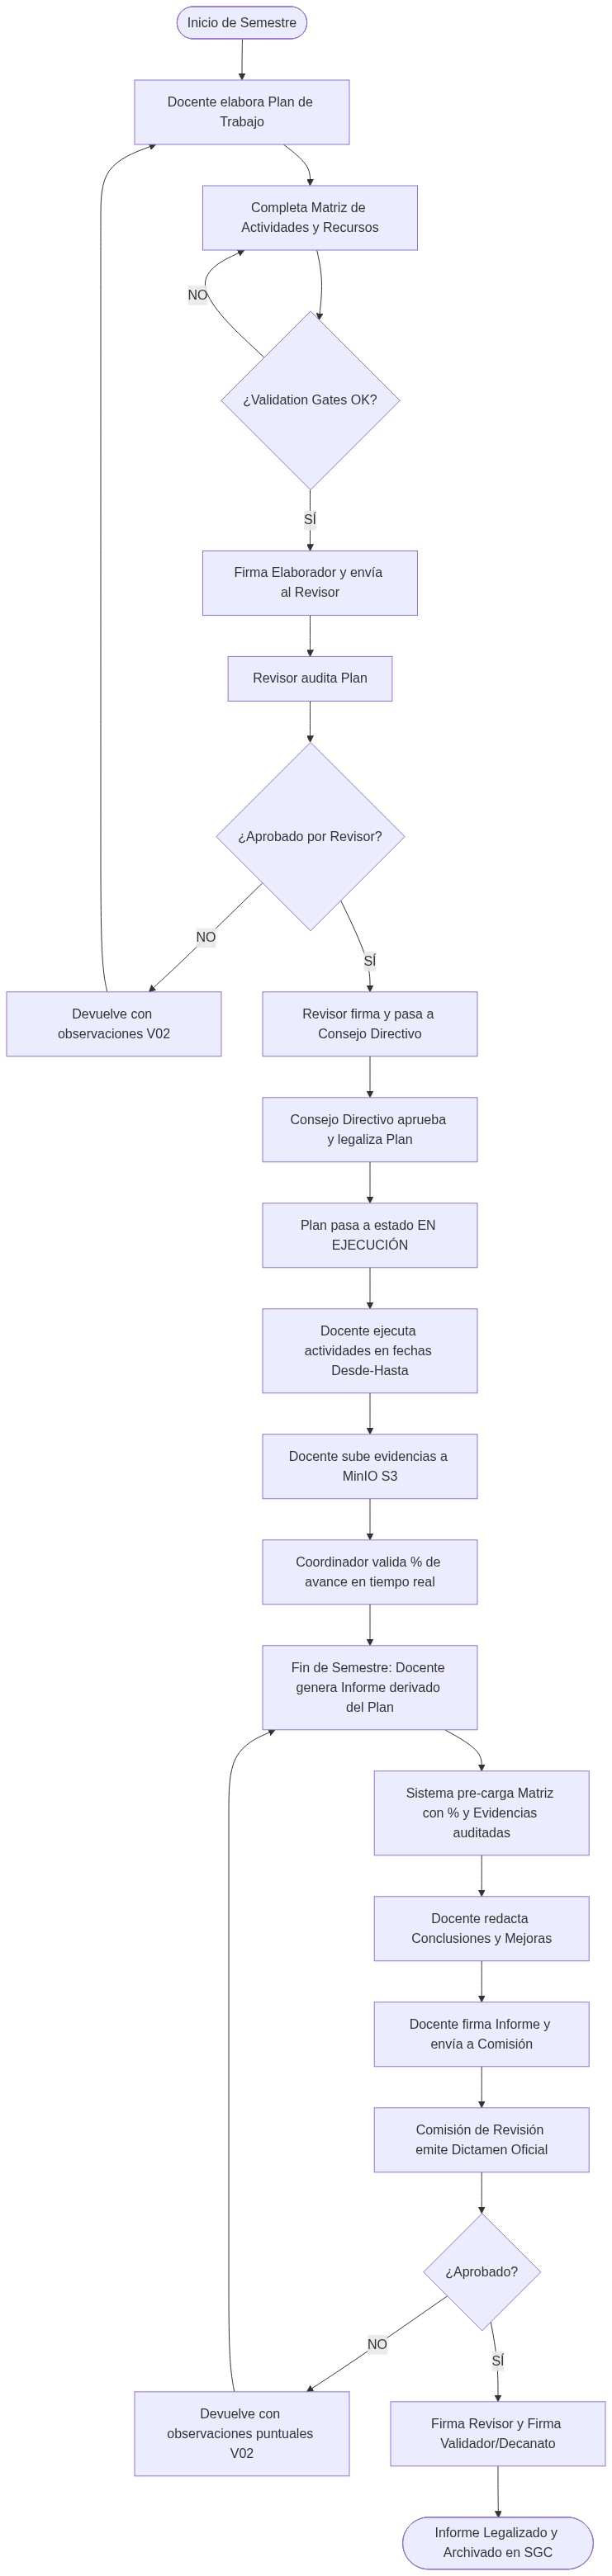
\includegraphics[width=0.88\textwidth,height=5.8cm,keepaspectratio]{images/s2_03_actividades_ciclo.png}
    \caption{Diagrama de Actividades UML: Ciclo Completo de Aprobación, Observación y Legalización.}
    \label{fig:actividades_ciclo}
\end{figure}
\FloatBarrier

\begin{figure}[H]
    \centering
    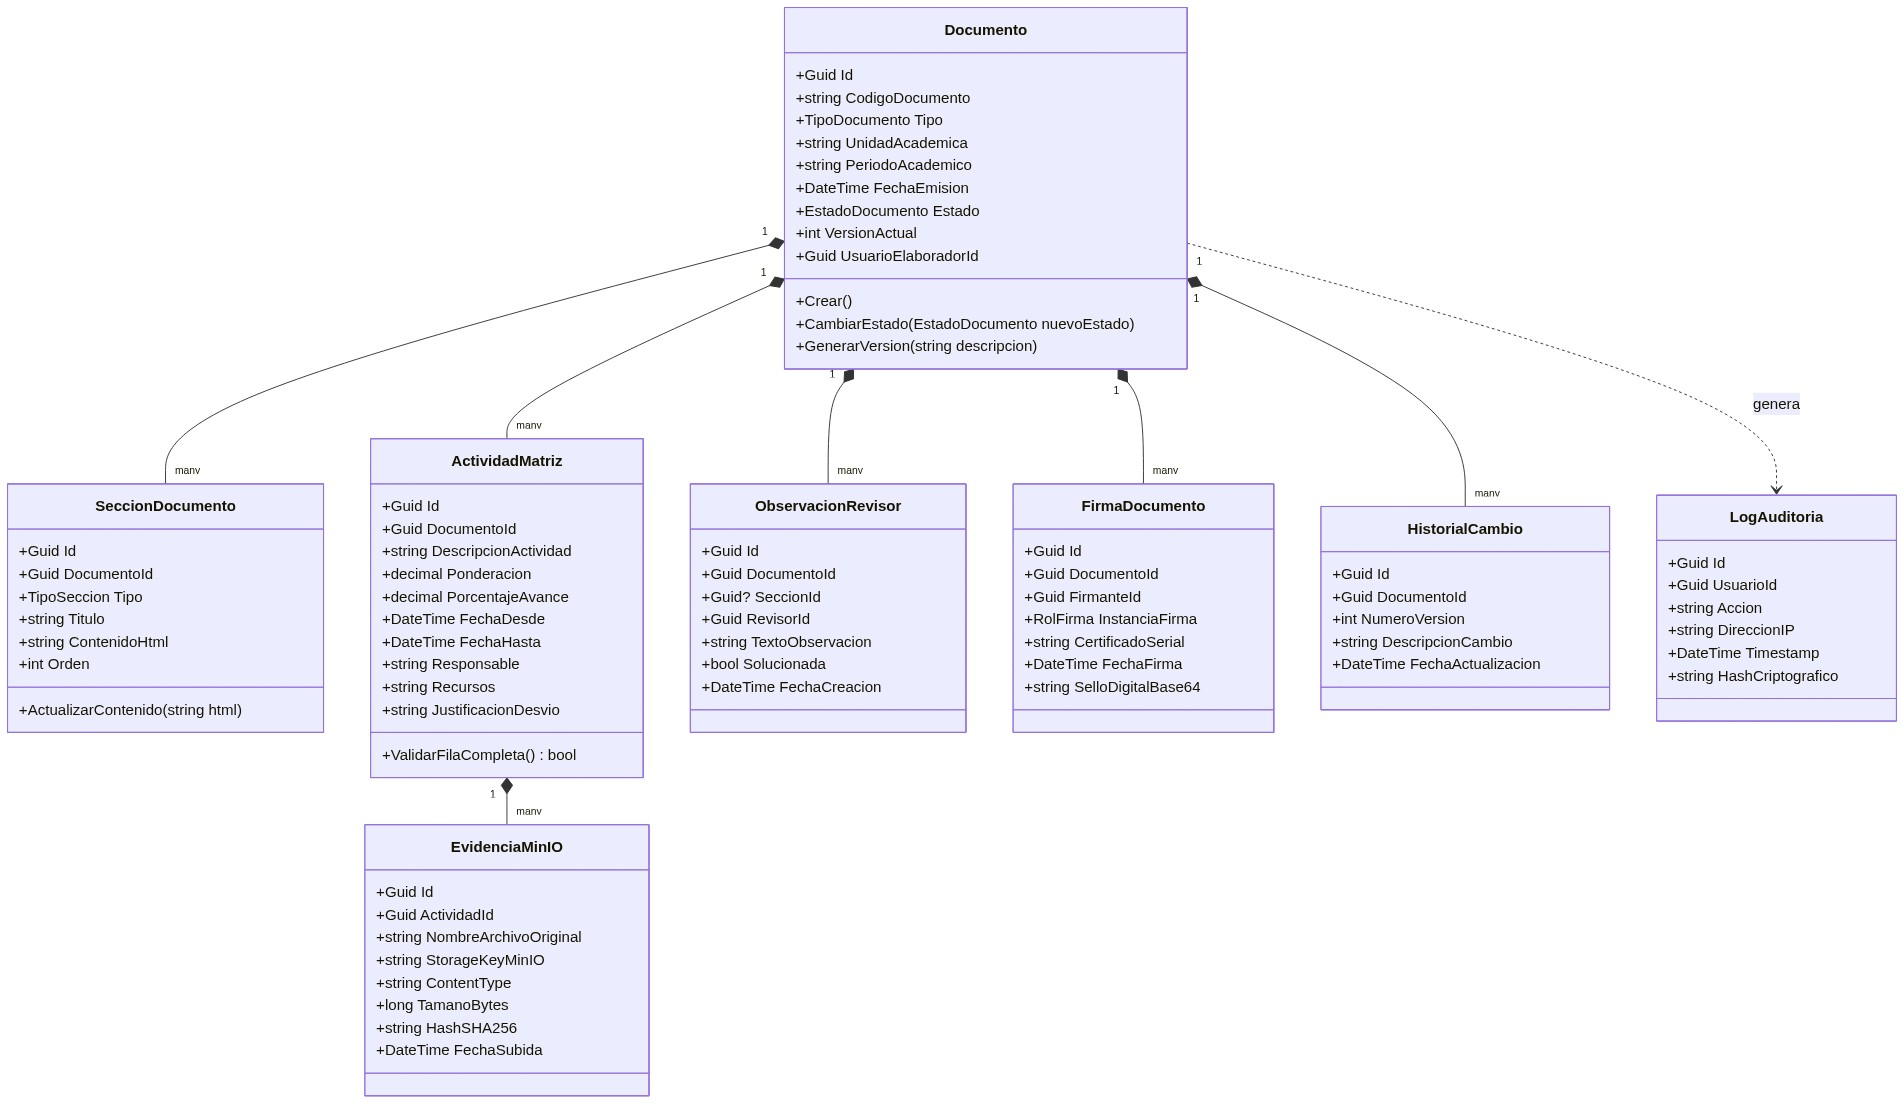
\includegraphics[width=0.88\textwidth,height=6.0cm,keepaspectratio]{images/s2_03_clases_uml.png}
    \caption{Diagrama de Clases del Dominio Institucional SIGE (Entidades, Atributos y Métodos).}
    \label{fig:clases_dominio}
\end{figure}
\FloatBarrier

\section{Descripción de actividades}
\subsection{Matriz de Entidades del Dominio y Métodos Operativos}
\begin{table}[H]
\centering
\small
\renewcommand{\arraystretch}{1.2}
\begin{tabularx}{\textwidth}{|>{\raggedright\arraybackslash\bfseries}m{3.2cm}|X|X|c|}
\hline
\rowcolor{tableheader}
\textbf{Clase de Dominio} & \textbf{Atributos Principales} & \textbf{Métodos de Negocio Clave} & \textbf{Multiplicidad} \\
\hline
\texttt{PlanDocente} & \texttt{id}, \texttt{periodo\_id}, \texttt{docente\_id}, \texttt{estado}, \texttt{horas\_totales} & \texttt{validarHorasMinimas()}, \texttt{avanzarEstado()}, \texttt{solicitarRevision()} & 1 \\
\hline
\texttt{SeccionDocumento} & \texttt{id}, \texttt{plan\_id}, \texttt{orden}, \texttt{titulo}, \texttt{contenido\_html} & \texttt{actualizarContenido()}, \texttt{sanitizarHtml()}, \texttt{bloquearEdicion()} & $1 \dots N$ \\
\hline
\texttt{ActividadMatriz} & \texttt{id}, \texttt{plan\_id}, \texttt{nombre}, \texttt{horas}, \texttt{ponderacion}, \texttt{cronograma} & \texttt{calcularAvance()}, \texttt{asignarMedio()}, \texttt{recalcularPonderacion()} & $1 \dots N$ \\
\hline
\texttt{EvidenciaAdjunta} & \texttt{id}, \texttt{actividad\_id}, \texttt{nombre\_archivo}, \texttt{url\_s3}, \texttt{hash\_sha256} & \texttt{verificarIntegridad()}, \texttt{generarUrlLectura()}, \texttt{asociarHash()} & $0 \dots N$ \\
\hline
\texttt{ObservacionComite} & \texttt{id}, \texttt{plan\_id}, \texttt{usuario\_id}, \texttt{seccion\_id}, \texttt{comentario}, \texttt{resuelto} & \texttt{registrarObservacion()}, \texttt{marcarResuelto()}, \texttt{auditarCambio()} & $0 \dots N$ \\
\hline
\texttt{FirmaDocumento} & \texttt{id}, \texttt{plan\_id}, \texttt{firmante\_id}, \texttt{rol\_firma}, \texttt{fecha\_firma}, \texttt{hash\_firma} & \texttt{estamparFirma()}, \texttt{validarSecuencia()}, \texttt{sellarDocumento()} & $0 \dots 3$ \\
\hline
\end{tabularx}
\caption{Matriz de especificación de clases del dominio SGC.}
\label{tab:espec_clases}
\end{table}

\subsection{Matriz de Transición de Estados del Documento Institucional}
\begin{table}[H]
\centering
\small
\renewcommand{\arraystretch}{1.2}
\begin{tabularx}{\textwidth}{|c|>{\raggedright\arraybackslash\bfseries}m{3.0cm}|X|X|}
\hline
\rowcolor{tableheader}
\textbf{Paso} & \textbf{Estado Inicial} & \textbf{Evento Disparador y Validación} & \textbf{Estado Resultante} \\
\hline
1 & \textit{Ninguno} & Creación de plan mediante asignación de periodo académico. & \textbf{Borrador} \\
\hline
2 & \textbf{Borrador} & Docente completa secciones y supera Validation Gates 1 a 4. & \textbf{En Revisión} \\
\hline
3 & \textbf{En Revisión} & Coordinador detecta inconsistencias y emite comentarios formales. & \textbf{Observado} \\
\hline
4 & \textbf{Observado} & Docente subsana observaciones y reenvía el documento. & \textbf{En Revisión} \\
\hline
5 & \textbf{En Revisión} & Coordinador de Área/Carrera aprueba y estampa su firma digital. & \textbf{Aprobado Comisión} \\
\hline
6 & \textbf{Aprobado Comisión} & Subdecano legaliza en Consejo Directivo y sella documento final. & \textbf{Aprobado HCD (Final)} \\
\hline
\end{tabularx}
\caption{Matriz de ciclo de vida de los estados del documento SGC.}
\end{table}

\section{Firmas de Responsabilidad}

\noindent
\renewcommand{\arraystretch}{1.2}
\begin{tabularx}{\textwidth}{|>{\raggedright\arraybackslash}m{2.9cm}|>{\raggedright\arraybackslash}X|>{\centering\arraybackslash}m{4.6cm}|>{\centering\arraybackslash}m{2.3cm}|}
    \hline
    \rowcolor{tableheader}
    \textbf{ACCIÓN} & \textbf{NOMBRE Y CARGO} & \textbf{FIRMA} & \textbf{FECHA} \\
    \hline
    \textbf{Elaborado por:} & Heidi Villavicencio\newline Analista de Calidad / UI-UX & \parbox[c]{4.4cm}{\centering\vspace{4pt}
\includegraphics[height=1.5cm,width=4.0cm,keepaspectratio]{images/firma_heidi.png}\vspace{4pt}} & 26/08/2026 \\
    \hline
    \textbf{Revisado por:} & Steeven Toala\newline Líder de Proyecto / Arquitecto & \parbox[c]{4.4cm}{\centering\vspace{4pt}
\includegraphics[height=1.5cm,width=4.0cm,keepaspectratio]{images/firma_steveen.png}\vspace{4pt}} & 26/08/2026 \\
    \hline
    \textbf{Aprobado por:} & Ing. Paulo Torres, Mg.\newline Docente Evaluador -- Gestión Proyectos & \parbox[c]{4.4cm}{\centering\vspace{8pt}\textbf{\textcolor{gray!80}{\scriptsize [ PENDIENTE DE APROBACIÓN ]}}\vspace{8pt}} & \textbf{\textcolor{gray!90}{Pendiente}} \\
    \hline
\end{tabularx}

\vspace{0.4cm}

\section{Control de Cambios}

\noindent
\renewcommand{\arraystretch}{1.2}
\begin{tabularx}{\textwidth}{|>{\hsize=0.45\hsize\centering\arraybackslash}X|>{\hsize=1.55\hsize\raggedright\arraybackslash}X|>{\hsize=1.2\hsize\raggedright\arraybackslash}X|>{\hsize=0.8\hsize\centering\arraybackslash}X|}
    \hline
    \rowcolor{tableheader}
    \textbf{Versión} & \textbf{Descripción del cambio} & \textbf{Responsable del cambio} & \textbf{Fecha de aprobación} \\
    \hline
    1.0 & Emisión inicial del entregable según EDT del Tablero Trello & Equipo de Proyecto SIGE & 26/08/2026 \\
    \hline
\end{tabularx}

\vspace{0.4cm}

\section{Anexos}

\subsection*{Anexo 1: Ficha Técnica de la Tarea EDT 2.3 en el Tablero Trello}
\begin{table}[H]
\centering
\small
\renewcommand{\arraystretch}{1.2}
\begin{tabularx}{\textwidth}{|>{\bfseries}m{3.5cm}|X|}
\hline
\rowcolor{tableheader}
\textbf{Parámetro EDT} & \textbf{Detalle Oficial del Tablero Trello} \\
\hline
Código de Tarea & EDT 2.3 \\
\hline
Nombre de la Tarjeta & Diagramas de secuencia, actividades y clases de dominio \\
\hline
Fase Correspondiente & FASE 2. DISEÑO Y ARQUITECTURA \\
\hline
Período de Ejecución & 21 de agosto al 26 de agosto de 2026 (4 días laborables) \\
\hline
Horas Asignadas & 32 horas hombre netas \\
\hline
Responsables Técnicos & Steeven Toala (ST), Andrea Vásquez (AV) \\
\hline
Entregable Oficial & \texttt{03\_Diagramas\_Secuencia\_Actividades\_Clases.pdf} \\
\hline
Estado en el Tablero & 100\% Completado y Aprobado en Reunión de Hito 2 \\
\hline
\end{tabularx}
\caption{Ficha técnica de la tarea EDT 2.3 en el Tablero Trello.}
\end{table}

\subsection*{Anexo 2: Definición Formal de Invariantes y Contratos de Dominio}
\begin{table}[H]
\centering
\footnotesize
\renewcommand{\arraystretch}{1.15}
\begin{tabularx}{\textwidth}{|c|m{3.2cm}|X|}
\hline
\rowcolor{tableheader}
\textbf{Invariante} & \textbf{Clase Responsable} & \textbf{Expresión Lógica del Contrato de Dominio} \\
\hline
INV-01 & \texttt{PlanDocente} & $\sum \text{horas\_actividad} \ge \text{horas\_minimas\_contrato}$ (40h tiempo completo). \\
\hline
INV-02 & \texttt{ActividadMatriz} & $\sum \text{ponderacion\_actividad} = 100.00\%$ al enviar a revisión. \\
\hline
INV-03 & \texttt{FirmaDocumento} & Secuencia estricta: $\text{Orden}(\text{Elaborador}) < \text{Orden}(\text{Revisor}) < \text{Orden}(\text{Aprobador})$. \\
\hline
INV-04 & \texttt{EvidenciaAdjunta} & $\text{Longitud}(\text{hash\_sha256}) = 64 \text{ caracteres hexadecimales}$ no nulos. \\
\hline
\end{tabularx}
\caption{Invariantes y contratos del modelo de dominio.}
\end{table}

\subsection*{Anexo 3: Trazabilidad en Repositorio Institucional Git}
\begin{itemize}[leftmargin=1.5em, itemsep=2pt]
    \item \textbf{Repositorio:} \texttt{FISEI\_Project / SIGE}
    \item \textbf{Rama de Trabajo:} \texttt{main}
    \item \textbf{Commit de Consolidación:} \texttt{b38190c - feat(arch): modelado dinamico UML, secuencia de gates y clases de dominio DDD}
    \item \textbf{Archivos Afectados:} \texttt{docs/diagramas\_dinamicos\_uml.md}, \texttt{Entregables\_Latex/Fase\_2/2.3*.tex}
\end{itemize}


\end{document}
